\documentclass [12pt, oneside, a4paper]{article}
\usepackage{color}
\usepackage{graphicx}
\usepackage{listings}
\usepackage{tikz}

\definecolor{mygreen}{rgb}{0,0.3,0}

\lstset{
  basicstyle=\footnotesize\ttfamily,
  keywordstyle=\footnotesize\bfseries\color{blue},
  numberstyle=\ttfamily\scriptsize,
  commentstyle=\itshape\color{mygreen},    % comment style
  tabsize=4,
  captionpos=b,
  frame=none,
  language=Verilog,
  %backgroundcolor=\color[rgb]{1,0.98,.98},
  breaklines=false,
  breakautoindent=false,
  postbreak=\space,
  breakindent=5pt,
  escapeinside={/*@}{@*/},
  aboveskip=3pt,
  belowskip=3pt,
  belowcaptionskip=0pt,
  morecomment=[l]{//},
  morekeywords={always, ifndef, define, endif},
  mathescape=true
}

\lstset{
  numbers=left, 
  frame=TRLB, 
  framexleftmargin=20pt, 
  xleftmargin=10pt, 
  numbersep=10pt
}

\lstdefinelanguage{z3}{
  keywords={declare-fun, assert, forall, not},
  morecomment=[l];,
  alsoletter=-,
}

\newcommand{\code}[1]{\texttt{#1}}
 
\begin{document}
	\begin{center}
	\textrm{\textbf{\LARGE Tutorial: SecVerilog}}\\[0.5cm]
	\rule{14cm}{1pt}\\[0.5cm]
	\textbf{Rui Xu\qquad Danfeng Zhang}\\[1mm]
	\today
	\end{center}
% Introduction of SecVerilog
SecVerilog~\cite{secverilog} is a new hardware description language (HDL) with
fine-grained information flow control. SecVerilog extends Verilog with
annotations that support comprehensive, precise reasoning about information
flows, including flows via timing, at compile time. The benefit is that
hardware designs can be verified mostly as-is, with little run-time overhead.

%Timing channels pose a real security risk, but methods are lacking for
%building systems without timing leaks. SecVerilog~\cite{secverilog}, combined with
%software-level enforcement, makes it possible to build systems in
%which timing channels and other leakage are verifiably controlled.
%SecVerilog extends Verilog with annotations that support
%comprehensive, precise reasoning about information flows at the
%hardware level. 
This tutorial assumes basic knowledge of using Verilog for hardware design. The
focus of this tutorial is on how to use SecVerilog to verify
information-flow security of hardware designs. 

The SecVerilog implementation is based on the open source tools
\code{Icarus Verilog (Iverilog)}~\cite{iverilog} (for compiling Verilog
modules), and Z3~\cite{z3} (for constraint solving). The extension to
Iverilog is included in the installation package of SecVerilog, while
you have to install Z3 separately.

% Installation of SecVerilog
\section{How to install SecVerilog}

You need to download the installation package, and uncompress the
package. The installation package contains two folders:

\begin{itemize}
\item \code{SecVerilog}: the SecVerilog compiler.

\item \code{Examples}: SecVerilog code examples.
\end{itemize}

In this tutorial, we refer to the first folder as \code{HOME} and the
second as \code{Example}. To build and install SecVerilog, execute the
following commands:

\begin{lstlisting}[language=bash, frame=none, numbers=none,
keywordstyle=\footnotesize\bfseries, morekeywords={make}]
cd HOME
./configure
make
make install
\end{lstlisting}

If you want SecVerilog being installed in a specified directory, say
\code{DIR}, use the following commands instead:

\begin{lstlisting}[language=bash, frame=none, numbers=none,
keywordstyle=\footnotesize\bfseries, morekeywords={make}]
cd HOME
./configure --prefix = DIR
make
make install
\end{lstlisting}

If all steps work well, SecVerilog is successfully installed
into the folder specified by the \code{DIR} parameter, or a default
folder (e.g., /usr/local/bin in Linux) when \code{prefix} is absent.
%The installation process needs to call the GCC compiler, and it
%requires versions that are higher or equal to 4.2. Lower versions of
%GCC may lead to compiler errors like: \code{call to `pow' is
%ambiguous}.  Therefore, you should make sure that your GCC compiler
%meets this restriction. 
The installation may require other packages, such as Gperf.  Please
install them when necessary.

\section{How to use SecVerilog}
\label{sec:usage}

We use the \code{oneway} example under the \code{Example} folder to
explain the usage of SecVerilog.

\begin{figure}
\begin{minipage}{.5\linewidth}
\begin{lstlisting}[framexbottommargin=25pt, language=z3, numbers=none,
framexleftmargin=0pt, xleftmargin=0pt]
; Domain(0)=L1, Domain(1)=L2
(declare-fun Domain (Int) Label)
(assert (= (Domain 0) L1))
(assert (= (Domain 1) L2))
\end{lstlisting}
\end{minipage}
\hfill
\begin{minipage}{.45\linewidth}
\begin{lstlisting}[language=z3, numbers=none,
framexleftmargin=0pt, xleftmargin=0pt]
; new lattice elements L1,L2
(declare-fun L1 () Label)
(declare-fun L2 () Label)

; lattice structure
(assert (leq L1 L2))
\end{lstlisting}
\end{minipage}
\caption{Declaration of type-level function (left) and lattice (right).}
\label{fig:oneway}
\end{figure}

\subsection{Invoke \code{iverilog} and \code{z3} binaries separately}

The \code{iverilog} binary takes Verilog files with security labels as
input, and produces a Z3 file as output. Besides the parameters of
Icarus Verilog, the \code{iverilog} command takes three new parameters:

\begin{itemize}
\item \code{-F depfunfile}: provide declarations of type-level functions. For
example, the left of Figure~\ref{fig:oneway} shows \code{EXAMPLE/oneway.fun}.
This file defines a type-level function \code{Domain}, where
\code{Domain(0)=L1} and \code{Domain(1)=L2}. Security levels \code{L1} and
\code{L2} are declared by the \code{-l} option as below.

\item \code{-l latticefile}: provide an extension to SecVerilog's
default security policy (in the form of a lattice of security levels).
By default, SecVerilog supports a ``diamond'' lattice with four
levels: \code{LOW}, \code{D1}, \code{D2} and \code{HIGH}. With the
extension on the right of Figure~\ref{fig:oneway}, the new security
policy forbids information from flowing ``down'' in the lattice below:

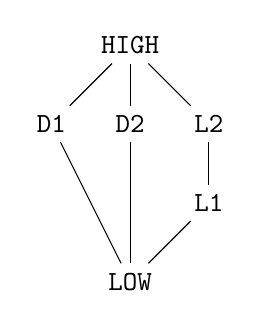
\begin{tikzpicture}
\node (H) {\code{HIGH}};
\node (D1) [left of=H, below of=H] {\code{D1}};
\node (D2) [right of=D1] {\code{D2}};
\node (L2) [right of=D2] {\code{L2}};
\node (L1) [below of=L2] {\code{L1}};
\node (L)  [left of =L1, below of=L1] {\code{LOW}};

\draw (H) -- (D1);
\draw (H) -- (D2);
\draw (L) -- (D1);
\draw (L) -- (D2);
\draw (H) -- (L2);
\draw (L2) -- (L1);
\draw (L1) -- (L);
\end{tikzpicture}

Note that by default, the new added labels are always lower than \code{High}
and higher than \code{Low}.

\item \code{-z}: verification only. That is, SecVerilog quits after
type-checking.
\end{itemize}

To verify program \code{oneway.v} in the folder \code{Example}, run
the following command in the \code{Example} folder:

\begin{lstlisting}[language=bash, frame=none, numbers=none,
keywordstyle=\footnotesize\bfseries, morekeywords={make}]
iverilog -F oneway.fun -l oneway.lattice -z oneway.v
\end{lstlisting}

The expected result is a Z3 file \code{oneway.z3} in the same folder.
Assume Z3 is already installed, the following command completes the
verification of file \code{oneway.v}:

\begin{lstlisting}[language=bash, frame=none, numbers=none,
keywordstyle=\footnotesize\bfseries, morekeywords={make}]
z3 -smt2 oneway.z3
\end{lstlisting}

For this example, the expected output is:
\begin{lstlisting}[language=bash, frame=none, numbers=none,
keywordstyle=\footnotesize\bfseries, morekeywords={make}]
unsat
unsat
unsat
sat
\end{lstlisting}

Here, \code{unsat} (\code{sat}) means the SecVerilog statement generating the
corresponding constraint is secure (insecure). Here, the last
constraint is generated by the last assignment in \code{oneway.v},
which is \code{d1 = d2}. Since the labels of \code{d1} and \code{d2}
are \code{L1} and \code{L2} respectively, an insecure flow from
\code{L2} and \code{L1} is correctly identified by SecVerilog in this
example.

\subsection{Use the \code{secverilog} script}

To ease the use of SecVerilog, the installation package contains a
Perl script template \code{secverilog.cp} under the folder
\code{Example}. The script can be used as is if both \code{iverilog}
and \code{z3} are under the PATH environment variable. Otherwise,
modify \code{\$z3home} and \code{\$iveriloghome} accordingly to the
binary folders of \code{z3} and \code{iverilog} respectively.

Once the template is configured properly and renamed as
\code{secverilog},  we can verify \code{oneway.v} by one command:

\begin{lstlisting}[language=bash, frame=none, numbers=none,
keywordstyle=\footnotesize\bfseries, morekeywords={make}]
./secverilog -F oneway.fun -l oneway.lattice -z oneway.v
\end{lstlisting}
or equivalently,
\begin{lstlisting}[language=bash, frame=none, numbers=none,
keywordstyle=\footnotesize\bfseries, morekeywords={make}]
perl secverilog -F oneway.fun -l oneway.lattice -z oneway.v
\end{lstlisting}

The expected output is:

\begin{lstlisting}[language=bash, frame=none, numbers=none,
keywordstyle=\footnotesize\bfseries, morekeywords={make}]
Compiling file oneway.v
Verifying file oneway.v
fail
(assert  (not(leq L2  L1)))    ; d1 = d2 @oneway.v:38
Total: 1 assertions failed
\end{lstlisting}

Here, the script clearly points to a security violation at line 38 of
\code{oneway.v}.

% Single file verification
\section{Design secure hardware with SecVerilog}

In this section, we create our very first {Verilog hardware module and
learn how to verify this module with SecVerilog. We use the two-input
mux hardware module shown in Figure~\ref{fig:blockdiagram} as a running
example. We start from building a RTL behavioral model, and then use
SecVerilog to verify its security.

\begin{figure}
\centering
\includegraphics[width=2.5in]{Two-Input-Mux.png}
\caption{Block diagram for a two-input mux: a mux module with two
one-bit input ports, a one-bit output port, and a one-bit select
control input.}
\label{fig:blockdiagram}
\end{figure}
%	\footnotesize{\textbf{Figure 1: Block Diagram for Two-input Mux} - A Mux module with two one-bit input port, a one-bit output port, and a one-bit select control input}}\\[0.1cm]
	
% RTL Behavioral Model
\subsection{RTL behavioral model of a two-input mux}

Figure~\ref{fig:twomux} shows the Verilog code which corresponds to the diagram in
Figure~\ref{fig:blockdiagram}. Lines 3-6 declare all parameters used
in the \code{Mux} module. \code{in1} and \code{in2} represent two
input ports. The \code{sel} variable controls which input signal can
be passed to the output port. Because this mux only has two
input ports, \code{sel} is a one-bit signal. The output port is
named \code{out}, which is also one-bit. Lines 11-16 model the
internal behavior of the module. When \code{sel} is zero, \code{in1}
is passed to the output port. Otherwise, the output port will select
the other input signal, \code{in2}.

% Establish Lattice Structure before security verification  
\subsection{Define a security policy}

To verify the security of a hardware design, we first need to define the
information-flow policy that the design should obey. Such policy is specified
as a lattice of security levels. A lattice of security levels restricts
information flow: information with lower security levels can flow to
information with higher security levels, but the opposite direction is
prohibited. 

Once a security lattice is defined, and information (variables) in the
hardware design is properly annotated with security labels, SecVerilog
can, at compile time, verify if the aforementioned information-flow
policy is enforced.

%structure actually defines the prinicples of information flow the
%module must follow. Any part of code, which violates defined policy,
%will be treated as insecure in SecVerilog.  Therefore, correctly
%building lattice structure is the base of verifying models with
%SecVerilog.

In order to specify the correct lattice structure for the module to be
verified, we need to figure out the security levels, and the
relationship between them. Returning to our running example, we assume
that there are three
different security levels, namely \code{D1} (domain 1), \code{D2} (domain 2),
and \code{LOW} (public) in this mux module. Any information flow between
\code{D1} and \code{D2} is not allowed. As the name of
indicates, \code{LOW} is the lowest secure level: information from this
level can be passed to any security levels including itself. However,
the opposite direction is prohibited.

%\setlength\fboxrule{2pt} 
% The example code for two input mux
\begin{figure}
\centering
%\framebox{\framebox{\parbox{.9\linewidth}{
\begin{minipage}{.8\linewidth}
\begin{lstlisting}
module Two_Input_Mux
(
	input in1,
	input in2,
	input sel,
	output out
);

reg	out;

always @ (*) begin
	if (sel == 1'b0)
		out = in1;
	else
		out = in2;
end
endmodule
\end{lstlisting}
\end{minipage}
%}}}
\caption{Two-Input mux: RTL behavioral code corresponding to the diagram in Figure~\ref{fig:blockdiagram}.}
\label{fig:twomux}
\end{figure}
%\footnotesize{\textbf{Figure 2: }}\\[0.2cm]

%\begin{center}
%	\framebox{\framebox{\parbox{.9\linewidth}{
%		\texttt{1\quad\quad \textcolor{red}{\`ifndef}\quad\quad Two\_Input\_Mux\_V \\
%				2\quad\quad \textcolor{red}{\`define}\quad\quad Two\_Input\_Mux\_V \\
%				3\\
%				4\quad\quad \textcolor{blue}{module}\quad\quad Two\_Input\_Mux \\
%				5\quad\quad \{ \\
%				6\quad\quad\quad\textcolor{blue}{input} \quad\quad\quad\quad in0; \\
%				7\quad\quad\quad\textcolor{blue}{input} \quad\quad\quad\quad in1; \\
%				8\quad\quad\quad\textcolor{blue}{input} \quad\quad\quad\quad sel;  \\
%				9\quad\quad\quad\textcolor{blue}{output}\quad\quad\quad\quad out \\
%				10\quad\quad\} \\
%				11 \\ 
%				12\quad \ \textcolor{blue}{reg} \quad\quad\quad\quad\quad\quad out;\\
%				13\\
%				14\quad \ \textcolor{blue}{always} \textcolor{red}{@(*)} \textcolor{blue}{begin}\\
%				15\quad \ \quad\textcolor{blue}{if} ( sel == 1`b0 ) \\
%				16\quad \ \quad\quad  out = in0; \\
%				17\\
%				18\quad \ \quad\textcolor{blue}{else} \\
%				19\quad \ \quad\quad out = in1; \\
%				20\quad \ \textcolor{blue}{end} \\
%				21\quad \ \textcolor{blue}{endmodule} \\
%				22\quad \ \textcolor{red}{\`endif}\quad\quad Two\_Input\_Mux\_V
%				}}}}\\[0.1cm]
%\end{center}
%\footnotesize{\textbf{Figure 2: Two-Input Mux} - RTL Behavioral code corresponding to the diagram in Figure 1}}\\[0.2cm]

The proper lattice is defined in a lattice file. For this example, the
security lattice is part of the default lattice in SecVerilog already. So no
lattice file is needed.
%The file responsible for the lattice structure is called \code{typecheck.cc}
%under the main directory.
The default lattice is declared by the code in Figure~\ref{fig:lattice}.
Lattice declaration has two parts --- lattice elements (security levels) and
lattice structure. Here, lines 2--5 declare four security levels:
\code{LOW}, \code{HIGH}, \code{D1} and \code{D2}. The relation among these
levels are specified by lines 8 and 9. Line 8 specifies that \code{LOW} is the
lowest (least restrictive) level among all levels, meaning that information
with \code{LOW} can flow to all levels. The dual of \code{LOW} is \code{HIGH},
where all information can flow into, as specified in line 9.

\begin{figure}
\centering
\begin{minipage}{.8\linewidth}
\begin{lstlisting}[language=z3]
; lattice elements
(declare-fun LOW () Label)
(declare-fun HIGH () Label)
(declare-fun D1 () Label)
(declare-fun D2 () Label)

; lattice structure
(assert (forall ((x label)) (leq LOW x)))
(assert (forall ((x label)) (leq x HIGH)))
\end{lstlisting}
\end{minipage}
\caption{Lattice structure for the two-input mux module.}
\label{fig:lattice}
\end{figure}
%\begin{center}
%	\framebox{\framebox{\parbox{0.9\linewidth}{
%		\texttt{1\quad\quad out << endl << \textcolor{blue}{``;  lattice elements'' } << endl;\\[0.1cm]
%			  2\quad\quad  out << \textcolor{blue}{``(declare-fun LOW () Label)''} << endl;\\[0.1cm]
%			  3\quad\quad  out << \textcolor{blue}{``(declare-fun HIGH () Label)''} << endl;\\[0.1cm]
%			  4\quad\quad  out << \textcolor{blue}{``(declare-fun D1 () Label)''} << endl;\\[0.1cm]
%			  5\quad\quad  out << \textcolor{blue}{``(declare-fun D2 () Label)''} << endl;\\[0.1cm]
%			  6\quad\quad \\[0.1cm]
%			  7\quad\quad  out << endl << \textcolor{blue}{``; lattice structure''} << endl;\\[0.1cm]
%			  8\quad\quad  out << \textcolor{blue}{``(assert (forall ((x label)) (leq LOW x)))''} << endl;\\[0.1cm]
%			  9\quad\quad  out << \textcolor{blue}{``(assert (forall ((x label)) (leq x HIGH)))''} << endl;\\[0.1cm]
%			 10\quad \        out << \textcolor{blue}{``(assert (not (= HIGH LOW))) ; the lattice cannot clapse''} << endl;\\[0.1cm]
%			 11\quad \ 	      out << \textcolor{blue}{``(assert (not (= D1 D2))''} << endl;\\[0.1cm]
%			 12\quad \       out << \textcolor{blue}{``(assert (not  (= LOW D1)))''} << endl;\\[0.1cm]
%			 13\quad \	      out << \textcolor{blue}{``(assert (not  (= LOW D2)))'' }<< endl;\\[0.1cm]
%	}}}}\\[0.5cm]
%	{\footnotesize{\textbf{Figure 3: Lattice Structre for Two-Input Mux module }}}
%\end{center}

%Verifying Two-Input Mux Using SecVerilog
\subsection{Verifying the two-input mux module}

In this example, the security concern is that inputs from different security
levels are fed to corresponding domains, with a shared output signal. The module
needs to avoid inputs from \code{D1} flowing to \code{D2}, and vise versa. In
another word, at each clock cycle, the input signal's level should be
consistent with that on the output port. So the following restrictions should
be obeyed:
\begin{itemize}
	\item Input \code{in1} belongs to \code{D1}
	\item Input \code{in2} belongs to \code{D2}
	\item Ouput \code{out}'s domain depends on the value of the signal \code{sel}. If the \code{sel} is zero, \code{out} belongs to \code{D1}. Otherwise, it belongs to \code{D2} 
\end{itemize}

%With defined lattice structure and above assumptions, we now begin to testify
%the secure characteristics of the mux module. We need to figure out what assets
%need to be protected. 
Figure~\ref{fig:sectwomux} presents the SecVerilog code for the
two-input mux (available as \code{EXAMPLE/mux.v}).
Compared to Figure~\ref{fig:twomux}, the baseline Verilog code, the only
difference is the security labels for variable declarations. SecVerilog uses
braces to denote security labels. In the simplest case, a security label is
simply a security level in the security lattice. For example, at line 3,
\code{\{D1\}} indicates that the input signal \code{in1} belongs to \code{D1}.

More interesting is the label of \code{out}, which depends on the run-time
value of \code{sel}. At line 6, \code{Domain} represents a type-level function,
which maps 0 to \code{D1} and 1 to \code{D2}. This type-level function is
declared in a separate function file, \code{EXAMPLE/diamond.fun}, as shown in
Figure~\ref{fig:diamond}.  Here, the declaration is very
straightforward: the first line declares a function named ``Domain'', and the
rest two lines specifies the desired mapping.

In general, the security labels in SecVerilog can be an application of
type-level functions, such as the label \code{\{Domain sel\}} for
\code{out}. This label exactly captures the restrictions on
\code{out}'s value: when \code{sel} is zero, \code{out} belongs to \code{D1};
when \code{sel} is one, \code{out} belongs to \code{D2}.

% The example SecVerilog code for two input mux
\begin{figure}
\centering
\begin{minipage}{.8\linewidth}
\begin{lstlisting}
module Two_Input_Mux
(
	input {D1}          in1,
	input {D2}          in2,
	input {L}           sel,
	output {Domain sel} out
);

reg	{Domain sel} out;

always @ (*) begin
	if (sel == 1'b0)
		out = in1;
	else
		out = in2;
end
endmodule
\end{lstlisting}
\end{minipage}
\caption{SecVerilog code of the two-input mux example: SecVerilog
version code for the two-input mux module in Figure~\ref{fig:twomux}.}
\label{fig:sectwomux}
\end{figure}

\begin{figure}
\centering
\begin{minipage}{.8\linewidth}
\begin{lstlisting}[framexbottommargin=0pt, language=z3, numbers=none,
framexleftmargin=0pt, xleftmargin=0pt]
; Domain(0)=D1, Domain(1)=D2
(declare-fun Domain (Int) Label)
(assert (= (Domain 0) D1))
(assert (= (Domain 1) D2))
\end{lstlisting}
\end{minipage}
\caption{Type-Level function \code{Domain} for the two-input mux example.}
\label{fig:diamond}
\end{figure}

%\begin{center}
%	\framebox{\framebox{\parbox{0.9\linewidth}{
%		\texttt{1\quad\quad \textcolor{red}{\`ifndef}\quad\quad Two\_Input\_Mux\_Sec\_V\\
%			  2\quad\quad \textcolor{red}{\`define}\quad\quad Two\_Input\_Mux\_Sec\_V\\
%			  3\\
%			  4\quad\quad \textcolor{blue}{module}\quad\quad Two\_Input\_Mux\_Sec \\
%			  5\quad\quad \{ \\
%			  6\quad\quad\quad \textcolor{blue}{input}\quad\quad \{D1\}\quad\quad\quad\quad\quad \ in0; \\
%			  7\quad\quad\quad \textcolor{blue}{input}\quad\quad \{D2\}\quad\quad\quad\quad\quad \ in1; \\
%			  8\quad\quad\quad \textcolor{blue}{input}\quad\quad \{L\}\quad\quad \ \quad\quad\quad \ sel; \\
%			  9\quad\quad\quad \textcolor{blue}{output}\quad \  \{Domain sel\} \quad out; \\
%			  10\quad\quad \}\\
%			  11\\
%			  12\quad\quad \ \textcolor{blue}{reg}\quad\quad\quad \{Domain sel\} \quad out; \\
%			  13\quad\quad \ \textcolor{blue}{always}\quad \textcolor{red}{@ (*)}\quad \textcolor{blue}{begin}\\
%			  14\quad\quad\quad \ \textcolor{blue}{if}  ( sel == 1`b0 )\\
%			  15\quad\quad\quad\quad \ out = in0;\\
%			  16\\
%			  17\quad\quad\quad \ \textcolor{blue}{else}\\
%			  18\quad\quad\quad\quad \ out = in1;\\
%			  19\quad\quad \ \textcolor{blue}{end}\\
%			  20\quad\quad \ \textcolor{blue}{end module}\\
%			  21\quad\quad \ \textcolor{red}{\`endif}\quad\quad Two\_Input\_Mux\_Sec\_V
%	}}}}
%\end{center}
%\footnotesize{\textbf{Figure 4: SecVerilog code of Two-Input Mux} - SecVerilog version code for Two-Input Mux Module in Figure 2}}\\[0.1cm]

%In the ideal situations, designers only add label to each parameter to complete SecVerilog version. However, adding labels is not enough in some situations, which will be discussed in the rest of the tutorial. 
The next step is to compile the above code with SecVerilog, and use
the \code{Z3 solver} to verify whether is there any violation of
the security policy. As described in Section~\ref{sec:usage}, this can
be done as follows:

\begin{lstlisting}[language=bash, frame=none, numbers=none,
keywordstyle=\footnotesize\bfseries, morekeywords={make}]
iverilog -F diamond.fun -z mux.v
z3 -zmt2 mux.z3
\end{lstlisting}

The expected output is a series of \textbf{\code{unsat}}, meaning that
there is no security violation in the SecVerilog code being analyzed.
For better debugging support, we recommend the ``secverilog'' script
for verification. As described in Section~\ref{sec:usage}, we can
simply run the following command to verify \code{mux.v}:
\begin{lstlisting}[language=bash, frame=none, numbers=none,
keywordstyle=\footnotesize\bfseries, morekeywords={make}]
perl secverilog -F diamond.fun -z mux.v
\end{lstlisting}

The expected output is:

\begin{lstlisting}[language=bash, frame=none, numbers=none,
keywordstyle=\footnotesize\bfseries, morekeywords={make}]
Compiling file mux.v
Verifying file mux.v
verified
Total: 0 assertions failed
\end{lstlisting}

%SecVerilog checks all assignment operations in consequence of the
%code. If any assignment go against the requirement of security, the
%result will be marked as \textbf{\code{sat}}. In the setting of
%SecVerilog, \textbf{\code{unsat}} means secure and \textbf{\code{sat}}
%implies insecure.

%However, the above way is inconvenient for designers to find out where
%the bugs are. The results only show that whether the assignment is
%secure or not rather than why it is insecure. Besides, designers have
%to count manually to figure out which assignment operation in the code
%violates the security restriction. Considering these inconvenience, we
%have written a script, named as \code{check.pl.cp} to ease the process
%of debugging. \code{Note: The script is written by perl. So you need
%to install perl firstly in order to run the script.} Before executing
%this script, we need to modify some parameters' value in the script to
%suit for our own computers:

%\begin{lstlisting}[language=bash, frame=none, numbers=none,
%keywordstyle=\footnotesize\bfseries, morekeywords={make},
%mathescape=false]
%Line 5   my $z3hone = ``path of z3 solver in your computer''
%Line 7   my $iverilog = ``path of iverilog in your computer''
%Line 23  my @files = (``the files's name you want to verify'')
%\end{lstlisting}

%Then we can run the script. If the parameters in the script is set
%correctly, the verification should display the information including
%how many assertions fail, where these failed assertions are and why
%they fail. In addition, designers can enter multiple files in the
%option of \code{my @files}, and verify these files at one turn rather
%than several times.

% Advanced use of SecVerilog
\section{Advanced use of SecVerilog}

The two-input mux example illustrates the basic usage of SecVerilog.
This part discusses some advanced aspects of SecVerilog, which may be
useful for advanced users.

% Define mapping function for dynamic labels
\subsection{User-Defined lattice and type-level functions}

SecVerilog supports arbitrary user-defined lattice structures and
type-level functions. They are defined in separate files and fed to
SecVerilog by parameters \code{-l} and \code{-F} respectively.

By default, SecVerilog supports a ``diamond'' lattice with four
labels: \code{LOW}, \code{D1}, \code{D2} and \code{HIGH}. With
extensions, such as the right of Figure~\ref{fig:oneway}, new lattice
elements (security levels) can be added in straightforward ways.

By default, SecVerilog supports a type-level function \code{LH}, which
maps 0 to \code{LOW}, and 1 to \code{HIGH}. With extensions, such as
the left of Figure~\ref{fig:oneway}, new functions can be added in
straightforward ways as well.

\begin{figure}
\centering
\begin{minipage}{.8\linewidth}
\begin{lstlisting}[language=z3]
(declare-fun Domain (Int) Label)
(assert (= (Domain 0) D1))
(assert (= (Domain 1) D2))
(assert (= (Domain 2) HIGH))
\end{lstlisting}
\end{minipage}
\caption{The Example Code of Defining Mapping Function \code{Domain}}
\label{fig:domaindef}
\end{figure}
%\begin{center}
%	\framebox{\framebox{\parbox{0.9\linewidth}{
%		\texttt{1\quad\quad out << \textcolor{blue}{``(declare-fun Domain (Int) Label)''} << endl;\\[0.1cm]
%			 2\quad\quad  out << \textcolor{blue}{``(assert (= (Domain 0) D1))'' } << endl;\\[0.1cm]
%			 3\quad\quad  out << \textcolor{blue}{``(assert (= (Domain 1) D2))'' } << end;\\[0.1cm]
%			 4\quad\quad  out << \textcolor{blue}{``(assert (= (Domain 2) HIGH))''} << endl;
%	}}}}\\[0.5cm]
%	\footnotesize{\textbf{Figure 5: The Example Code of Defining Mapping Function \code{Domain}}}
%\end{center}
% Rewriting logic for SecVerilog
\subsection{Rewrite hardware designs for SecVerilog}

In the ideal case, designers only need to add security labels for
variable declarations, if the hardware design being verified is
secure. However, due to the imprecision of SecVerilog's type
system\footnote{Such imprecision mostly comes from the program
analyses adopted in the current implementation of SecVerilog.}, secure
designs sometimes need to be slightly modified to overcome such
imprecision.
 
One way to overcome such limitation is to add extra conditions to rule
out impossible states. Next, we illustrate such limitation by
examples.

%Implicit Information Flow of if\else Syntax
\subsubsection{Reasoning about impossible states}

For security, SecVerilog must conservatively consider all possible
hardware states that might occur at run time. However, sometimes, the
hardware designers write Verilog code in a way that gets the design
away from insecure circumstances. In general, it is hard for
SecVerilog to reason about the impossibility of such insecure states
at compile time. We use the example in Figure~\ref{fig:impflow} to
illustrate this situation.

The left of Figure~\ref{fig:impflow} shows a secure design, which is
(incorrectly) rejected by SecVerilog. In this example, the module
selectively passes the input request \code{req} to \code{req\_low}
with label \code{LOW}, or \code{req\_d1} with label \code{Domain1}, or
\code{req\_d2} with label \code{Domain2}, according to the value of
\code{sel}. Here, the type-level function \code{Domain} maps 0 to
\code{L}, 1 to \code{D1}, and 2 to \code{D2}.

This design is secure because the signal \code{sel} only holds three
possible values (0, 1, 2). This is enforced in other pieces of code.
In another word, in the last branch of the source code, the security
level of \code{req} must be \code{D2}. Therefore, there is no
security violation in this program. However, since SecVerilog needs to
consider all possibilities, including the impossible case where
\code{sel} is 3, this program is rejected.

The right of Figure~\ref{fig:impflow} shows a functionally equivalent
hardware design, which can be verified by SecVerilog. The only added
code is the branch condition for the last branch. Such added condition
helps SecVerilog to rule out the impossible insecure state, so that
the design passes the SecVerilog verification.

\begin{figure}
\begin{minipage}{.49\linewidth}
\begin{lstlisting}[numbers=none, framexleftmargin=0pt]
input [1:0] {L}  sel;
input [3:0] {L}  req_low;
input [3:0] {D1} req_d1;
input [3:0] {D2} req_d2;
//Domain 0=L, 1=D1, 2=D2
output[3:0] {Domain sel} req;
if (sel == 0)
	req_low = req;
else if (sel == 1)
	req_d1 = req;
else
	req_d2 = req;
\end{lstlisting}
\end{minipage}
\hfill
\begin{minipage}{.49\linewidth}
\begin{lstlisting}[numbers=none, framexleftmargin=0pt]
input [1:0] {L}  sel;
input [3:0] {L}  req_low;
input [3:0] {D1} req_d1;
input [3:0] {D2} req_d2;
//Domain 0=L, 1=D1, 2=D2
output[3:0] {Domain sel} req;
if (sel == 0)
	req_low = req;
else if (sel == 1)
	req_d1 = req;
else if (sel == 2)
	req_d2 = req;
\end{lstlisting}
\end{minipage}
\caption{Rewriting hardware designs to aid SecVerilog.}
\label{fig:impflow}
\end{figure}

%Change of Interface due to labels
\subsubsection{Reason about invariants}

Another source of imprecision is the failure of SecVerilog to reason
about invariants established in hardware designs. We use the example
in Figure~\ref{fig:change} to illustrate this case.

In this example, the type-level function maps 0 to \code{D1} and 1 to
\code{D2}.  The code on the left seems insecure, because when
\code{sel} is 1, the assignment to \code{do\_enq} effectively leaks
information with label \code{D2} (the value of \code{enq\_rdy}) to the
security domain \code{D1} (\code{do\_enq}). However, this design is
secure because the hardware designer restricts \code{enq\_val} to be
zero whenever \code{sel} is 1. Therefore, the value of \code{do\_enq}
is always zero whenever \code{sel} is 1---no information is leaked
from \code{D2} to \code{D1}.

To aid SecVerilog to observe the relation of \code{sel} and
\code{enq\_val}, we can rewrite the code on the left as the one shown
on the right of Figure~\ref{fig:change}. The aforementioned invariant
is now explicit in the rewritten code, so that SecVerilog correctly
accepts this program.

\begin{figure}
\begin{minipage}{.49\linewidth}
\begin{lstlisting}[numbers=none, framexleftmargin=0pt, framexbottommargin=36pt]
input  {D1} enq_val;
input  {Domain sel} enq_rdy;
input  {L}  sel;
output {D1} do_enq;
assign do_enq = enq_val 
              & enq_rdy;
\end{lstlisting}
\end{minipage}
\hfill
\begin{minipage}{.49\linewidth}
\begin{lstlisting}[numbers=none, framexleftmargin=0pt]
input  {D1} enq_val;
input  {Domain sel} enq_rdy;
input  {L}  sel;
output {D1} do_enq;
if (sel == 1'b0)
	do_enq = enq_val 
	       & enq_rdy;
else
	do_enq = 1'b0;
\end{lstlisting}
\end{minipage}
\caption{Change of interface leads to added code.}
\label{fig:change}
\end{figure}

% Matters need attention
\section{Limitations in current implementation}

The current implementation of SecVerilog has the following
limitations. 

% list of situation needing attention
\begin{itemize}
\item  SecVerilog does not allow adding labels to the \code{parameter}
data type. One workaround is to turn these types into \code{input} ports with
constant values.

\item  When sub-modules are in the same file with a main module, these
sub-modules are not verified by SecVerilog. One workaround is to put
sub-modules in separate files.

%\item  For projects including multiple \textit{Verilog} files,
%designers need to contain all files in the scripts
%during the process of verification. If you only include the
%highest-level file in the script, SecVerilog
%will only check the interface between the highest-level module and the
%next-level modules. It will not check
%whether the internal logic in next-level modules is secure or not.
%Therefore, in order to make sure the whole
%design is secure, designers should include all related files in the
%script. 
\item  For dynamic labels, inputs for a mapping function must be a
complete variable. SecVerilog does not support a dependency on certain
bits of a variable yet. For example, a label \code{\{Domain x[0]\}} is
not allowed.

\item Each bit in a variable must have the same label.  

\item  SecVerilog currently does not support \code{task} and
\code{function}. Such code blocks will be ignored during verification.
Designers can inline these blocks, or turn these blocks into
\code{module}s to avoid this limitation.
\end{itemize}

\begin{thebibliography}{3}
\bibitem{iverilog}
{{I}carus {V}erilog}.
\newblock http://iverilog.icarus.com/.

\bibitem{z3}
L.~M. de~Moura and N.~Bj{\o}rner.
\newblock {Z3}: An efficient {SMT} solver.
\newblock In {\em Proc. Conf. on Tools and Algorithms for the Construction and
  Analysis of Systems (TACAS)}, 2008.

\bibitem{secverilog}
D.~Zhang, Y.~Wang, G.~E. Suh, and A.~C. Myers.
\newblock A Hardware Design Language for Timing-Sensitive Information-Flow Security.
\newblock In {\em Proc. 20th Int'l Conf. on Architectural Support for
Programming Languages and Operating Systems (ASPLOS)}, 2015. 
\end{thebibliography}

\end{document}
